% !TeX encoding = UTF-8
% !TeX root = choix_extensions.tex
\chapter{Gérer les graphiques}
\label{ch:graphiques}





\section{Texte et figure en parallèle}



\subsection{Figure sans légende - raccourcis}

Le fichier \lstinline!preambule_college.sty! contient des raccourcis basés sur les \lstinline!minipage! : \newline
\lstinline!\txtfig{taille_texte en %}{texte}{figure}! et \lstinline!\figtxt{taille_figure en %}{figure}{texte}! :


%\setlength\fboxsep{0pt}
%\setlength{\txtWidth}{(\linewidth - \widthof{\quad}) * \real{.65}}
%\setlength{\figWidth}{\linewidth - \widthof{\quad} - \txtWidth }
%\noindent
%\begin{minipage}[m]{\txtWidth}
%	{Texte en parallèle d'une figure.}
%\end{minipage}% %N.B. le % est nécessaire pour éviter un espace inter-mot supplémentaire entre les minipages
%\hfill
%\begin{minipage}[m]{\figWidth}
%	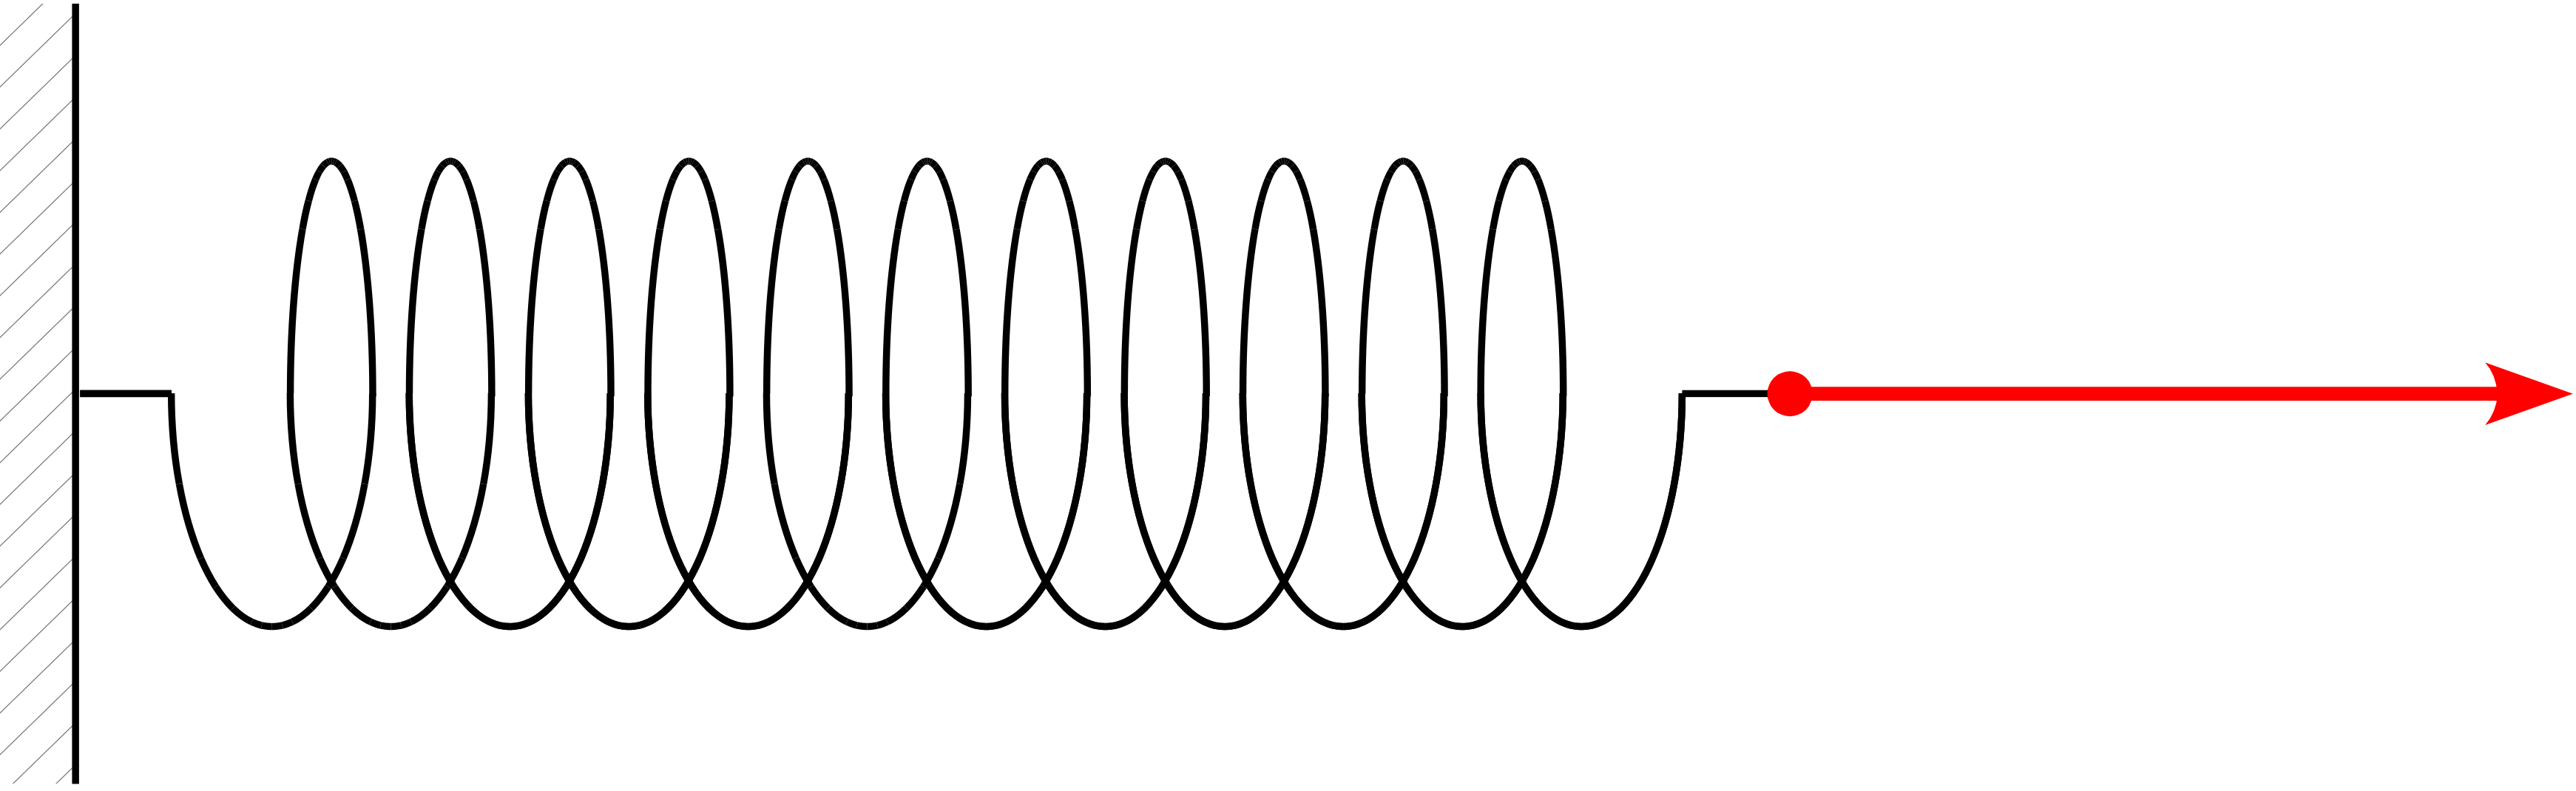
\includegraphics[width=\linewidth]{images/vecteur_force}
%\end{minipage}


\begin{LTXexample}[pos=o]
\txtfig{.65}
  {Texte en parallèle d'une figure.}
  {images/vecteur_force}
\end{LTXexample}

\begin{LTXexample}[pos=o]
\figtxt{.65}
  {images/vecteur_force}
  {Texte en parallèle d'une figure.}
\end{LTXexample}


\subsection{Figure sans légende - à la main}

Presque la même, mais à la main : on peut ainsi jouer sur les paramètres de centrage des minipages. Par exemple, ici avec le paramètre \lstinline![m]! (milieu) :

\begin{LTXexample}[pos=o]
\begin{minipage}[m]{.58\linewidth}
    Texte en parallèle d'une figure.
\end{minipage}% %Un % est nécessaire ici
\hfill
\begin{minipage}[m]{.38\linewidth}
    \centering
%    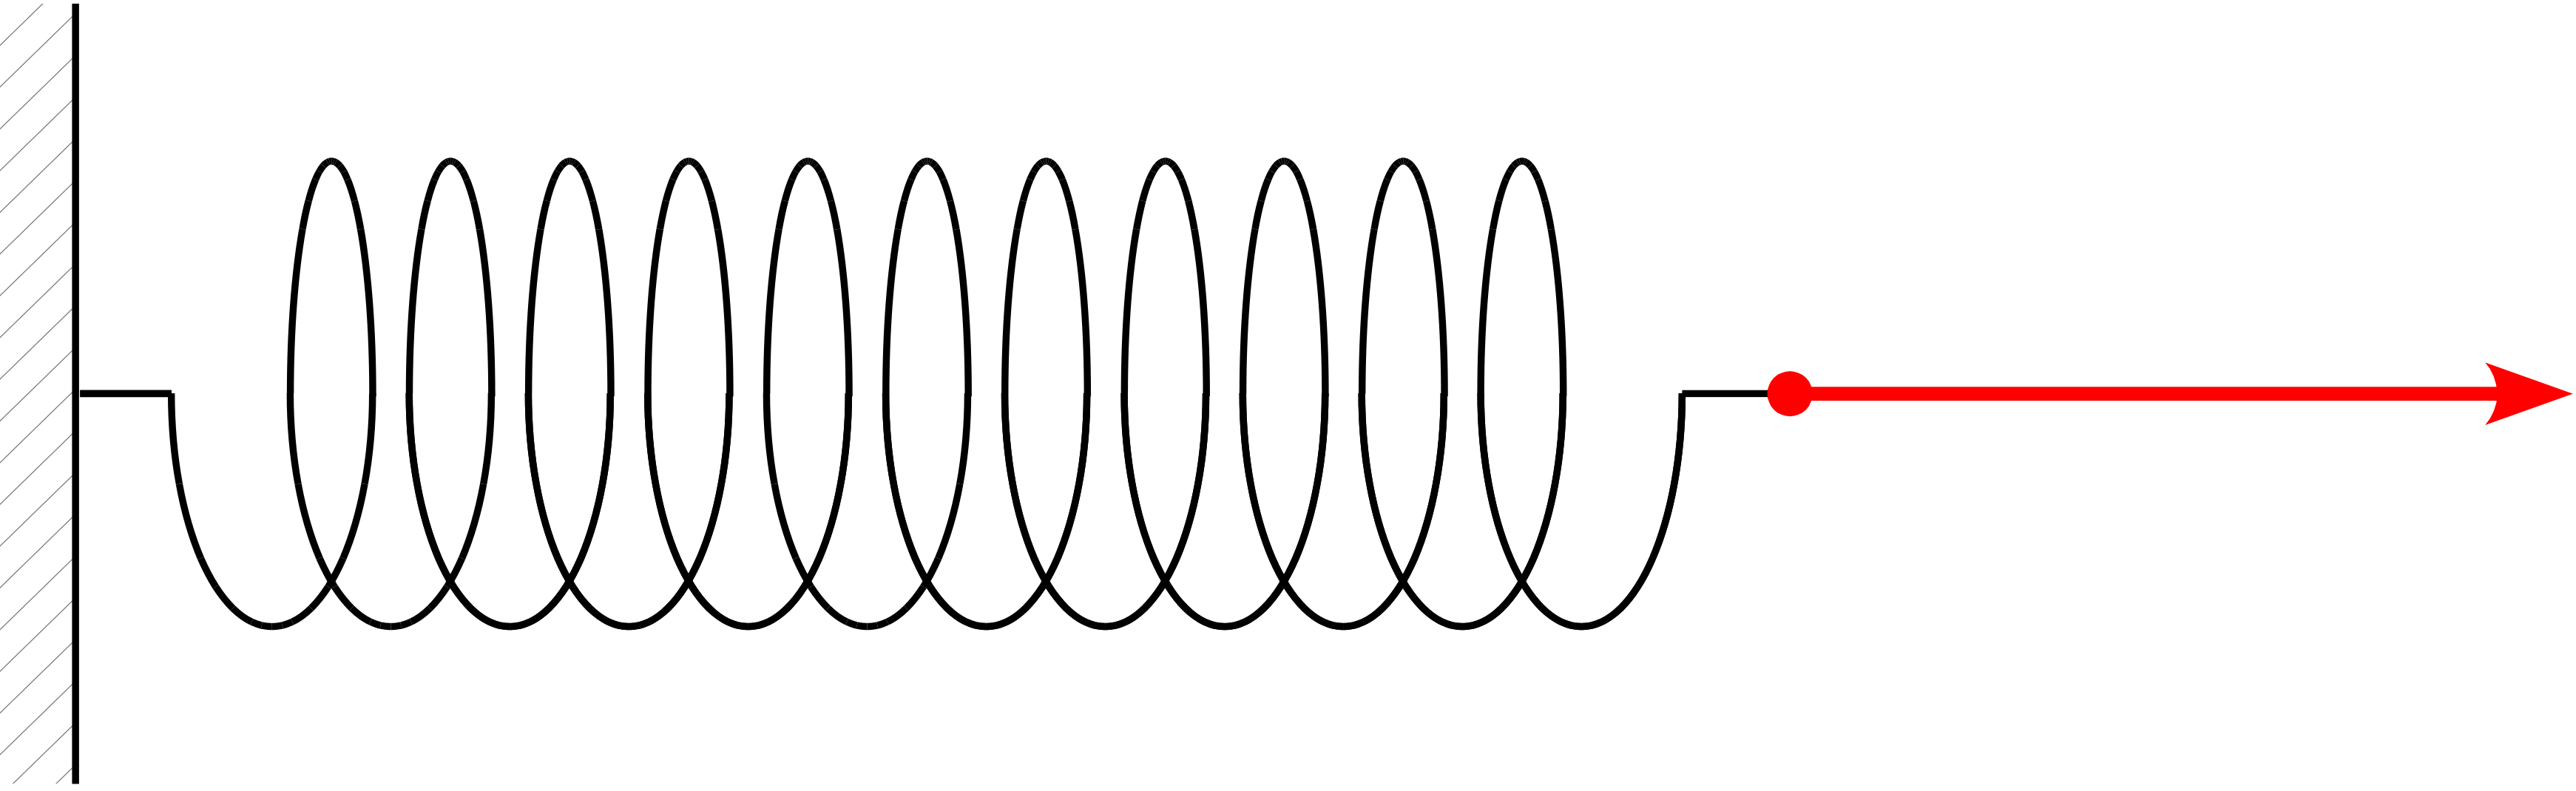
\includegraphics[width=\linewidth]{images/vecteur_force}
\end{minipage}
\end{LTXexample}



\subsection{Figure avec légende}

\begin{LTXexample}[pos=o]
\begin{minipage}[m]{.58\linewidth}
    Texte en parallèle d'une figure.
\end{minipage}% %Un % est nécessaire ici
\hfill
\begin{minipage}[m]{.38\linewidth}
    \centering
%    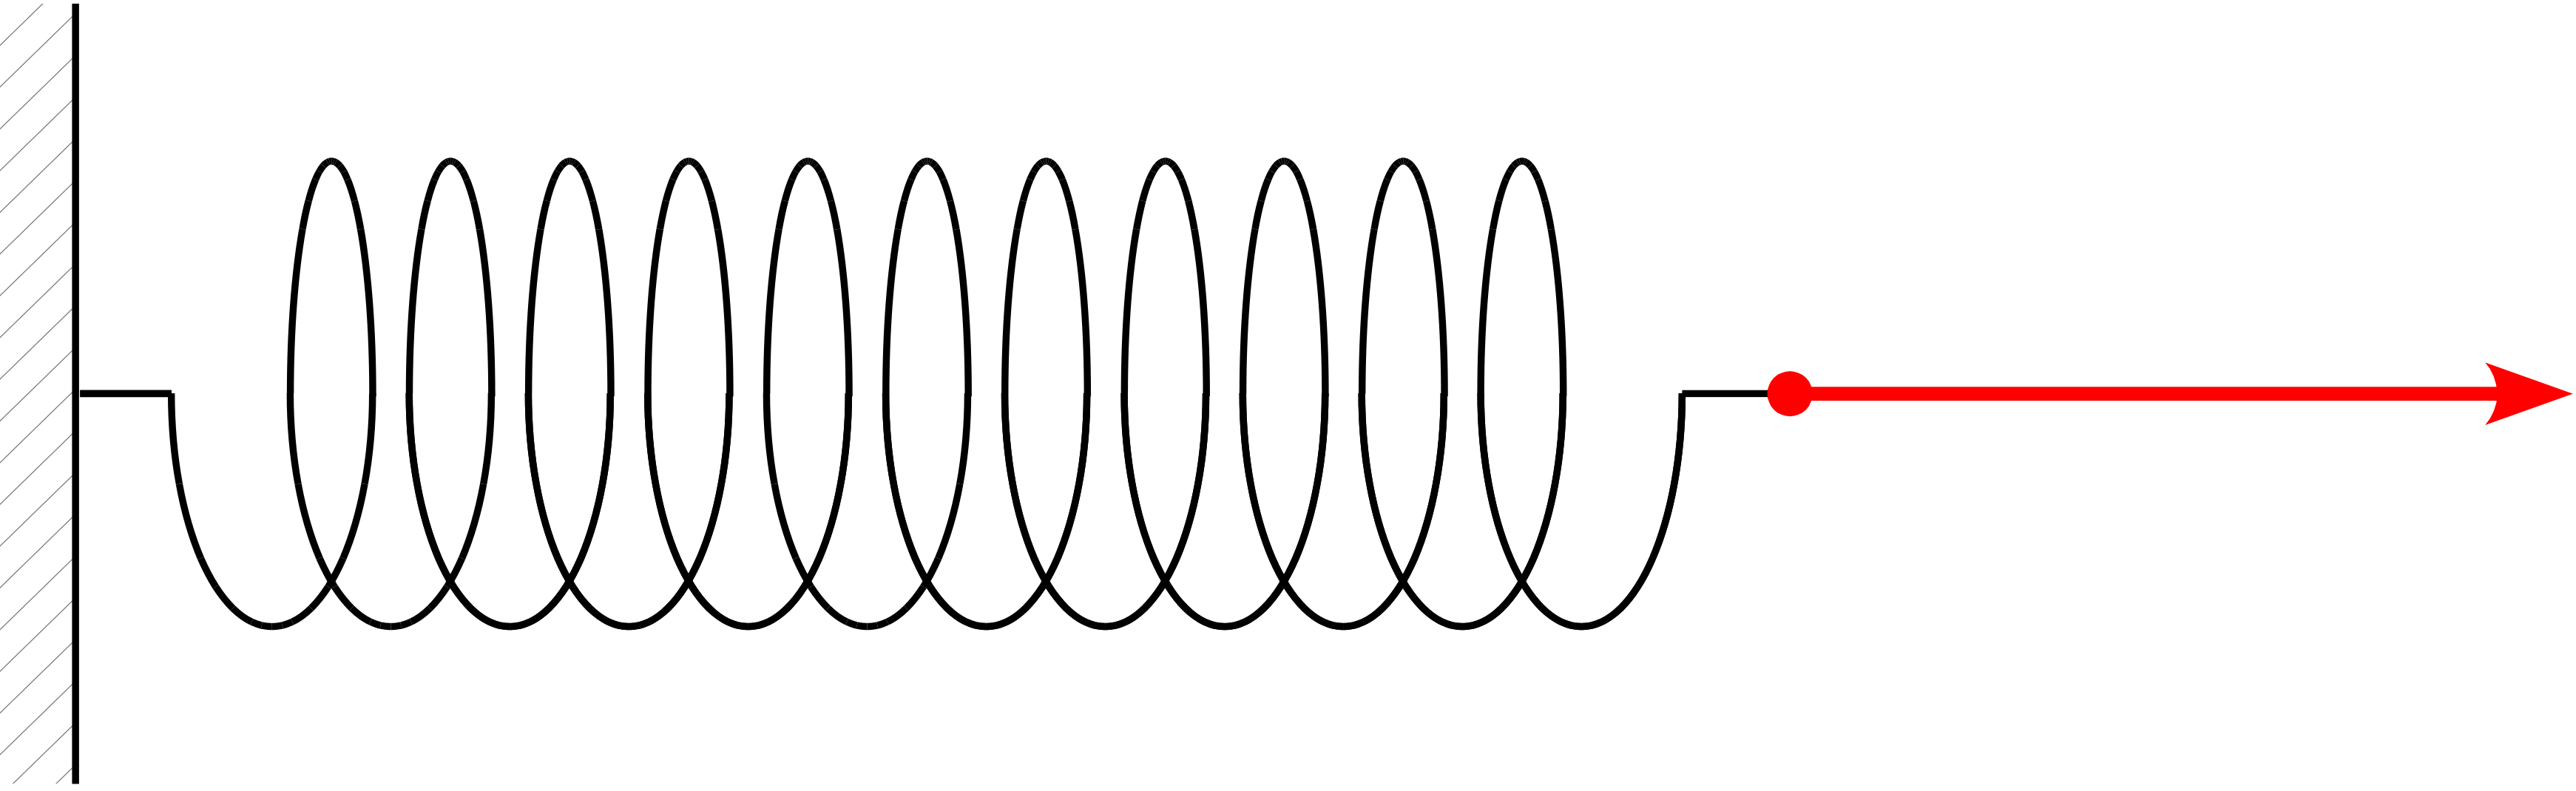
\includegraphics[width=\linewidth]{images/vecteur_force}
    \captionof{figure}{Force}
\end{minipage}
\end{LTXexample}

\remarques*{
	\listtopsep
	\begin{enumerate}
		\item Attention \mintinline{latex}{\captionof{figure}{...}} de l'extension \href{http://www.ctan.org/pkg/caption}{caption} permet d'insérer une légende dans une minipage, mais peut chambouler l'ordre de la numérotation pour les figures à proximité. Il faut vérifier le placement des autres figures autour de celle-ci.
		\item On peut aussi faire ce type de mise en page avec l'extension \mintinline{latex}{float} et \mintinline{latex}{\begin{figure}[H]}, mais ceci n'est pas entièrement compatible avec l'usage de l'extension \mintinline{latex}{minitoc}.
	\end{enumerate}
}





\section{Sous-figures}
\label{sec:textFig}

\begin{minipage}[m]{.48\linewidth}
	\begin{minted}{latex}
\begin{figure}{\linewidth}
  \centering
  \captionsetup{type=figure}
  \subcaptionbox
    {Lentille biconvexe\label{fig:l1}}
    [.45\linewidth]
    {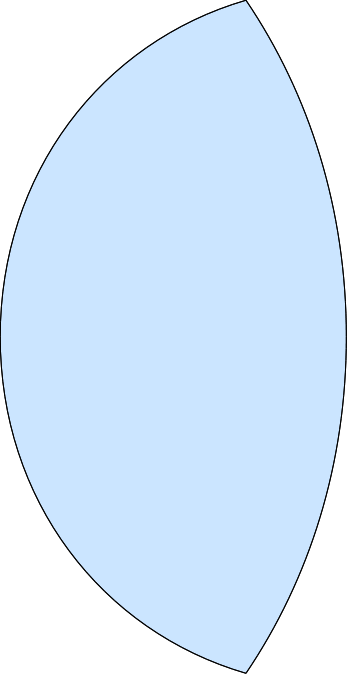
\includegraphics{images/lentille1}
  }
  \quad
  \subcaptionbox
    {Ménisque à bord mince\label{fig:l2}}
    [.45\linewidth]{
    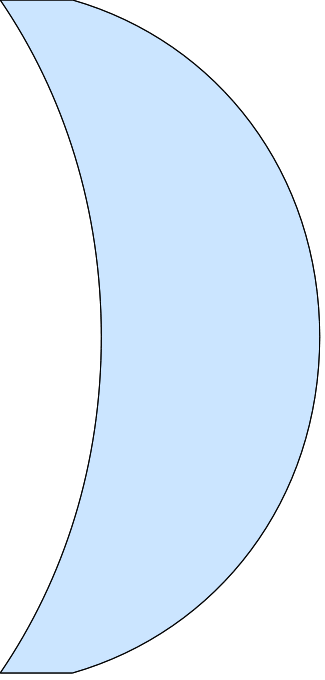
\includegraphics{images/lentille2}
  }
  \caption{Lentilles convergentes
  	\subref{fig:l1} et \subref{fig:l2}}
  \label{fig:lentillesTypes}
\end{figure}
	\end{minted}
\end{minipage}
\hfill
\begin{minipage}[m]{.48\linewidth}
	\begin{figure}[H]%{\linewidth}
		\centering
		\captionsetup{type=figure}
		\subcaptionbox{Lentille biconvexe\label{fig:l1}}[.45\linewidth]{
			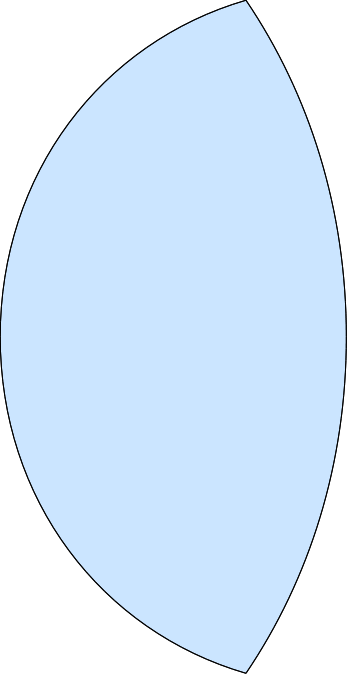
\includegraphics{images/lentille1}
		}
		\quad
		\subcaptionbox{Ménisque à bord mince\label{fig:l2}}[.45\linewidth]{
			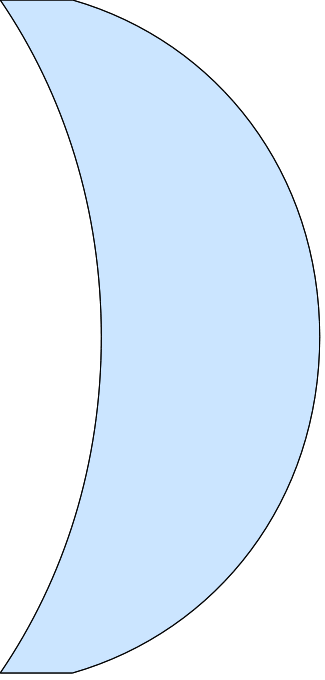
\includegraphics{images/lentille2}
		}
		\caption{Lentilles convergentes
			\subref{fig:l1} et \subref{fig:l2}}
		\label{fig:lentillesTypes}
	\end{figure}
\end{minipage}


\remarque*{
	L'extension \mintinline{latex}{\href{http://mirror.ctan.org/macros/latex/contrib/subfig/subfig.pdf}{subfig}} permet aussi de faire ce type de mise en page, mais elle a des incompatibilités avec \mintinline{latex}{hyperref}.
%	\begin{minipage}[m]{.48\linewidth}
%		\begin{minted}{latex}
%	\begin{figure}[H]
%	  \centering
%	  \subfloat[Lentille biconvexe]{
%	    \includegraphics[width=2.5cm]
%	      {images/lentille1}}
%	    \label{a}
%	   }
%	  \quad
%	  \subfloat[Ménisque à bord mince]{
%	    \includegraphics[width=2.5]
%	      {images/lentille2}
%	     }
%	    \label{b}
%	  }
%	  \caption{Lentilles convergentes}
%	  \label{fig:lentillesTypes}
%	\end{figure}
%		\end{minted}
%	\end{minipage}
%	\hfill
%	\begin{minipage}[m]{.48\linewidth}
%		\begin{figure}[H]
%			\centering
%		  	\subfloat[Lentille biconvexe]{
%		    \makebox[2.5cm]{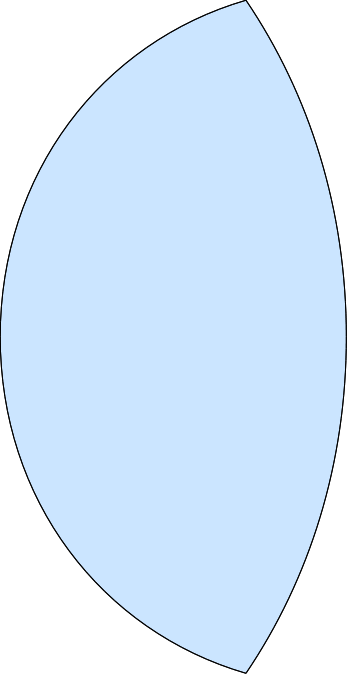
\includegraphics{images/lentille1}}
%		    \label{a}
%		  }
%		  \quad
%		  \subfloat[Ménisque à bord mince]{
%		    \makebox[2.5cm]{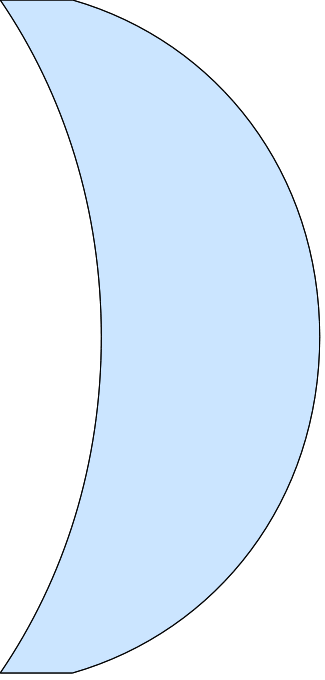
\includegraphics{images/lentille2}}
%		    \label{c}
%		  }
%		  \caption{Lentilles convergentes}
%		  \label{fig:lentillesTypes}
%		\end{figure}
%	\end{minipage}
}





\section{Alignement horizontal des minipages}

Si on veut aligner correctement le haut de deux \mintinline{latex}{minipages} (deux options \mintinline{latex}{[t]}), il se peut que le résultat ne soit pas celui escompté (voir code ci-après) :

\begin{LTXexample}[pos=o,width=.4]
\begin{minipage}[t]{4cm}
  \[
    \cS_{B'CC'} = \cS_{B'BC'}
  \]
\end{minipage}
\hfill
\begin{minipage}[t]{2cm}
  \centering
  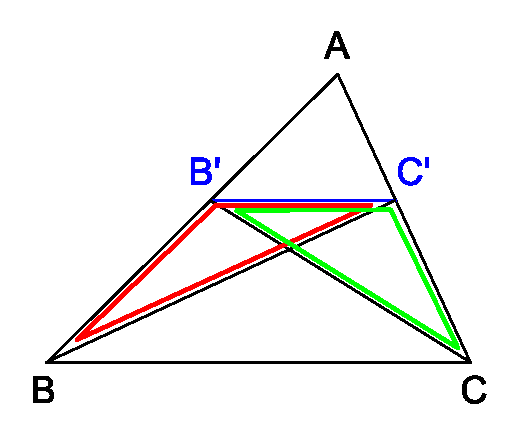
\includegraphics
    [width=.8\linewidth]
    {images/Thales_thm_Thales_dem_01}
\end{minipage}
\end{LTXexample}

Pour éviter cela, il suffit de rajouter \mintinline{latex}{\vspace{0pt}} dans la deuxième \mintinline{latex}{minipage} de manière à donner un point de référence correct à \LaTeX.

\begin{LTXexample}[pos=o,width=.4]
\begin{minipage}[t]{4cm}
  \[
    \cS_{B'CC'} = \cS_{B'BC'}
  \]
\end{minipage}
\hfill
\begin{minipage}[t]{2cm}
  \vspace{0pt}
  \centering
  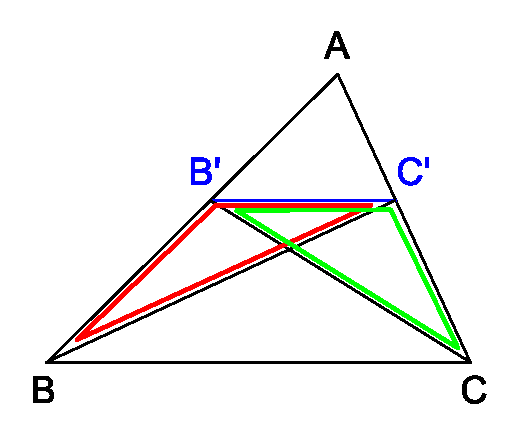
\includegraphics
    [width=.8\linewidth]
    {images/Thales_thm_Thales_dem_01}
\end{minipage}
\end{LTXexample}